\section{Indexed \ProbDef}
\label{index}

We propose to solve \probdef{} problem using an index based approach. This section describes how to process a \probdef{} query on a static graph, including \inducedgraph{} construction, creating \treeindex{}, performing various kind of queries on the preprocessed index. In the next section, we describe index update procedure on dynamic graphs.

\subsection{\InducedGraph{}}
\usernote{use counting sort}

We first design an \inducedgraph{} then propose the query algorithm based on it.

\vskip 0.1in \noindent \textbf{\InducedGraph{} Construction.} We first compute the edge trussness of graph $G_o$ and then construct a new graph $G_m$, which we called \inducedgraph{}, based on the graph $G_o$ and its edges' trussness. We define the \inducedgraph{} as follows.

\begin{Def}[\inducedgraph{}]
The \inducedgraph{} is a weighted maximum spanning forest that each edge $e$ in $G_o$ is represented as a vertex $x$ in $G_m$. An edge $y$ in $G_m$ represents that the two edges, which are represented by the two adjacent vertices of $y$, are contained in the same triangle in $G_o$. The weight of the each vertex in $G_m$ is its represented edge's trussness in $G_o$. The weight of each edge in $G_m$ is the lowest edge trussness of its related triangle's edges in $G_o$.
\label{def:\inducedgraph{}}
\end{Def}

We denote $G_{m}^{\prime}$ as the graph that is constructed the same way as $G_m$ but with all triangles in $G_o$ as edges, \ie $G_m$ is the maximum spanning forest of $G_{m}^{\prime}$. We refer to lowest edge trussness of a triangle as the weight of the triangle. 

We have the following theorem for vertex weights and edge weights in \inducedgraph{} $G_m$.

\begin{Thm}
In \inducedgraph{} $G_m$, for each vertex $x$ and each of its adjacent edge $y$, we have $w_x \ge w_y$.
\label{thm:\inducedgraph{}_vertex_trussness}
\end{Thm}

\begin{proof}
According to \autoref{def:\inducedgraph{}}, $w_x$ is the trussness of the represented edge $e$ in $G_o$ while $w_y$ is the lowest trussness of edges in the represented triangle $\triangle$ in $G_o$. We have $\tau_{e} \ge \tau_{\triangle}$, therefore, $w_x \ge w_y$.
\end{proof}

%\begin{algorithm}
	%\KwData{$G_{o}(V,E)$}
	%\KwResult{edge trussness $\{\tau_{e}, e \in E\}$}
	%\BlankLine
	%compute $s_e$ for each edge $e$ and sort in ascending order\;
	%$k \gets 2$\;
	%\While{$\exists e \in E$}{
		%\While{$\exists e$ such that $s_e \le k - 2$}{
			%$e \gets$ lowest support edge $(u, v)$\;
			%$u \gets$ lower degree end of $e$\;
			%\For{$w \in N_u$}{
				%\If{$(v,w) \in E$}{
					%$s_{(u,w)} \gets s_{(u,w)} + 1$\;
					%$s_{(v,w)} \gets s_{(v,w)} + 1$\;
					%reorder the sorted list of edges\;
				%}
			%}
			%$\tau_e \gets k$\;
			%remove $e$ from $E$\;
		%}
		%$k \gets k + 1$\;
	%}
	%\Return{$\{\tau_{e}, e \in E\}$}
	%\caption{Truss Decomposition}\label{alg:truss_decomposition}
%\end{algorithm}

%The truss decomposition algorithm \cite{wang2012truss} is used to compute trussness of all edges in $G_o$. For the ease of reader, we show the algorithm in \autoref{alg:truss_decomposition}. The algorithm first computes support of each edge by counting number of triangles it belongs to. Then, for $k$ starting at $2$, it iteratively removes the edge with lowest support from the graph and update supports of other edges accordingly. The removed edge is given the edge trussness of $k$. The algorithm increases $k$ by $1$ if there is no more edge has a support lower than $k - 2$. 
%The algorithm takes $O(\sum{(u,v) \in E}\min{d_u, d_v}$ time and $O(m)$ space for computing the trussness of all edges.

\begin{algorithm}
	\KwData{$G_{o}(V_{o},E_{o})$, edge trussness $\{\tau_{e}, e \in E_{o}\}$}
	\KwResult{$\inducedgraph{} G_{m}(V_{m}, E_{m})$}
	\BlankLine
	$visited \gets \emptyset$\;
	\For{$(u,v) \in E_{o}$}{
		suppose $u$ is the lower degree end of $(u,v)$\;
		$V_{m} \gets V_{m} \bigcup \{(u,v), \tau_{(u,v)}\}$\;
		\For{$w \in N_{u}$}{
			\If{$(v,w) \in E_{o}$ \textbf{and} $\triangle_{uvw} \notin visited$}{
				$visited \gets visited \bigcup \triangle_{uvw}$\;
				$\tau_{\triangle_{uvw}} = min(\tau_{(u,v)}, \tau_{(u,w)}, \tau_{(v,w)})$\;
				$V_{m} \gets V_{m} \bigcup \{(u,w), \tau_{(u,w)}\}$\;
				$V_{m} \gets V_{m} \bigcup \{(v,w), \tau_{(v,w)}\}$\;
				$E_{m} \gets E_{m} \bigcup \{((u,v),(u,w)), \tau_{\triangle_{uvw}}\}$\;
				$E_{m} \gets E_{m} \bigcup \{((u,v),(v,w)), \tau_{\triangle_{uvw}}\}$\;
				$E_{m} \gets E_{m} \bigcup \{((u,w),(v,w)), \tau_{\triangle_{uvw}}\}$\;
			}
		}
	}
	run Kruskal's algorithm on $G_m$\;
	\Return{$G_m$}
	\caption{\Inducedgraph{} construction}\label{alg:\inducedgraph{}_construction}
\end{algorithm}

The truss decomposition algorithm \cite{wang2012truss} is used to compute trussness of all edges $\{\tau_{e}, e \in E_{o}\}$ in $G_o$. Although it is possible to directly compute k-truss communities based on edge trussness with BFS traversals, such an algorithm suffers from high time complexity for redundant edge access~\cite{huang2014querying}. \autoref{alg:\inducedgraph{}_construction} uses both $G_o$ and edge trussness as inputs to construct the \inducedgraph{} $G_m$ for optimal query time. The algorithm iterates through all edges of $G_o$ and create a vertex in $G_m$ for each edge $(u,v)$ in $G_o$ with weight $\tau_{(u,v)}$. Then for each unvisited neighbor triangle $\triangle_{uvw}$ of edge $(u,v)$, the algorithm creates three edges $((u,v),(u,w))$, $((u,v),(v,w))$ and $((u,w),(v,w))$ in $G_m$ with same weight $\tau_{\triangle_{uvw}} = min(\tau_{(u,v)}, \tau_{(u,w)}, \tau_{(v,w)})$. After that, one can simply run Kruskal's algorithm to get the maximum spanning forest.

\begin{figure}[ht]
    \centering
    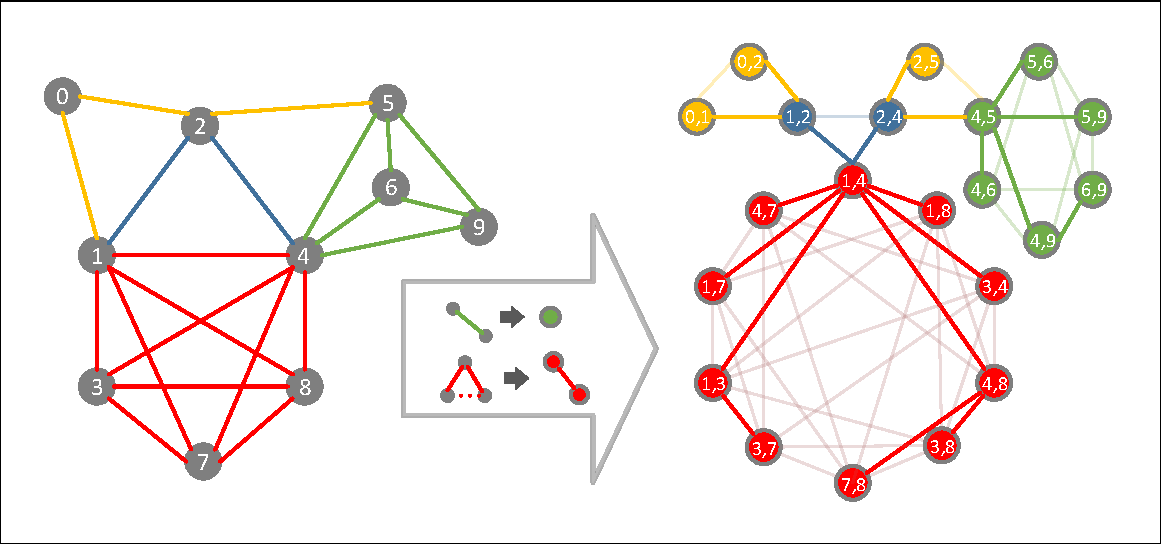
\includegraphics[width=\linewidth]{./figures/induced_graph.pdf}
    \caption{An example \inducedgraph{} of the example graph in \autoref{fig:example}}
    \label{fig:\inducedgraph{}}
\end{figure}

We show an example of \inducedgraph{} in \autoref{fig:\inducedgraph{}}. We outline the \inducedgraph{} of the example graph in \autoref{fig:example} with bold lines. The rest lines are edges that are generated by \autoref{alg:\inducedgraph{}_construction} but discarded by Kruskal's algorithm. 

\note{some possible error of time complexity in~\cite{huang2014querying}}
The time and space complexity for computation of edge trussness of $G_o$ are $O(\sum_{(u,v) \in E_{o}}{min\{d_{u},d_{v}\}})$ and $O(m)$ respectively~\cite{huang2014querying}. Listing all the triangles in $G_o$ takes $O(\sum_{(u,v) \in E_{o}}{min\{d_{u},d_{v}\}})$ time and $O(\sum_{(u,v) \in E_{o}}{min\{d_{u},d_{v}\}})$ space. Finally, running Kruskal's algorithm takes $O(\sum_{(u,v) \in E_{o}}{min\{d_{u},d_{v}\}}log{m})$ time. As $G_m$ is a maximum spanning forest, so the \inducedgraph{} index takes $O(|V_m|) = O(m)$ space.

\vskip 0.1in \noindent \textbf{Query on \InducedGraph{}.} To query the k-truss communities of a query vertex $q$ in $G_o$, the algorithm iterate through adjacent edges of the vertex $q$. For each neighbor edge $(u,q)$ that is unvisited by the algorithm, it is marked as a seed edge for a new community $C_i$. Suppose the edge $(u,q)$ in $G_o$ is represented as a vertex $x$ in $G_m$, the algorithm starts a BFS/DFS from vertex $x$ in $G_m$ and only expands through edges with weight $\ge k$ to find the connected component $CC$. Then if finds the represented edge $e$ of each vertex $v \in CC$ and adds $e$ to the community $C_i$. The union of all communities $A = \bigcup C_i$ is all the k-truss communities the vertex $q$ belongs to.

\begin{Thm}
The union of all communities $\bigcup C_i$ found by \autoref{alg:\inducedgraph{}_query} is the union of all the k-truss communities containing query vertex $q$.
\label{thm:\inducedgraph{}_query}
\end{Thm}

\begin{proof}
According to \autoref{def:\inducedgraph{}}, a vertex $x$ in \inducedgraph{} $G_m$ with weight $w_{x} \le k$ means the represented edge $e$ in $G_o$ has trussness $\tau_{e} \le k$ and thus can be included in a k-truss community. An edge $(x,y)$ in \inducedgraph{} $G_m$ with weight $w_{(x,y)} \le k$ means the represented triangle $\triangle$ in $G_o$ has all three edges with trussness higher or equal to $k$ and thus the triangle is included in a k-truss community containing all three edges of it. Adjacent edges in $G_m$ means adjacent triangles in $G_o$ and connected components in $G_m$ means triangle connected components in $G_o$. So, BFS/DFS search starts with a seed vertex $x$ with weight constraint will find the maximal connected component including $x$ which representing the k-truss community that $e$ belongs to in $G_o$ ($x$ represents $e$ in $G_m$). Therefore, performing such BFS/DFS searches on each edge of the query vertex will find all the k-truss communities that the query vertex belongs to.
\end{proof}

\begin{algorithm}
	\KwData{$G_{o}(V_{o},E_{o})$, $G_{m}(V_{m},E_{m})$, an integer $k$, a query vertex $q$}
	\KwResult{a union of all k-truss communities $\bigcup C_i$ containing $q$}
	\BlankLine
	$i \gets 0$, $visited \gets \emptyset$\;
	\For{$u \in N_{q}$}{
		\If{$(u,q) \notin visited$}{
			find representing vertex $x$ of $(u,q)$ in $G_m$\;
			$CC \gets$ connected component containing $x$ with edges of weight $\ge k$\;
			$C_i \gets \emptyset$\;
			\For{$v \in CC$}{
				find represented $e$ of $v$ in $G_o$\;
				$visited \gets visited \bigcup e$\;
				$C_i \gets C_i \bigcup e$\;
			}
			$i \gets i + 1$\;
		}
	}
	\Return{$\bigcup C_i$}
	\caption{Query on \inducedgraph{}}\label{alg:\inducedgraph{}_query}
\end{algorithm}

Since the query process is performing a BFS on a maximum spanning forest, each query takes $O(|A|)$ time and $O(|A|)$ space, where $|A|$ is the number of edges in $A$. Although such time complexity is already optimal if the detailed communities are required. We propose a new index structure that can be constructed upon the \inducedgraph{} to further reduce the time complexity if details of k-truss communities are not required.

\subsection{\TreeIndex{}}

We first show how to construct the \treeindex{} based on \inducedgraph{}. Then we design an algorithm to efficiently query the \treeindex{}. 

\vskip 0.1in \noindent \textbf{\TreeIndex{} Construction.} A key observation in~\cite{cohen2008trusses} is that, for $k \ge 2$, each k-truss of $G_o$ is the subgraph of a (k-1)-truss of $G_o$. With this observation, for k-truss communities, we have the following theorem.

\begin{Thm}
A k-truss community $C_k$ is the subgraph of a l-truss community $C_l$, if $C_k$ and $C_l$ are triangle connected and $l < k$. If k-truss community $C_k$ is the subgraph of both $l_1$-truss community $C_{l_1}$ and $l_2$-truss community $C_{l_2}$, then $l_1 \neq l_2$.
\label{thm:truss_hierarchy}
\end{Thm}

\begin{proof}
For the first part, since $l < k$, if edges in $C_k$ are triangle connected through triangles with trussness of $k$, then they are also triangle connected through triangles with trussness of $l$. 

\note{do we call it k-truss or $l_1$-truss.}
For the second part, suppose $l_1 = l_2$, then edges in $C_{l_1}$ and $C_{l_2}$ are triangle connected through $C_k$. So $C_{l_1} \bigcup C_{l_2}$ meets the definition of k-truss community (\autoref{def:k-truss_community}) and becomes a larger k-truss community. This contradicts with $C_{l_1}$ and $C_{l_2}$ are k-truss communities themselves, \ie they are maximal k-truss.
\end{proof}

\begin{algorithm}
	\KwData{$G_{m}(V_{m},E_{m})$}
	\KwResult{$G_{t}(V_{t},E_{t})$, $h$}
	\BlankLine
	$Q \gets \emptyset$, $parent \gets \emptyset$\;
	\While{$V_{m} \neq \emptyset$}{
		$seed \gets$ an unvisited vertex in $V_{m}$, $Q \gets Q \bigcup seed$\;
		\While{$Q \neq \emptyset$}{
			$x = Q.pop()$\;
			\For{$z \in N_x$}{
				$Q \gets Q \bigcup z$, $parent[z] \gets x$\;
			}
			\eIf{$x \in parent$}{
				$y \gets parent[x]$, $C_a \gets C_{y}^{max}$\;
				\While{$\tau_{C_a} > w_{(x,y)}$}{
					$C_c \gets C_a$, $C_a \gets$ parent of $C_a$ in $G_t$\;
					\If {$C_a = \emptyset$}{
						$\tau_{C_a} \gets -1$ \Comment{Reach the top of the tree.}\;
					}
				}
				\eIf{$\tau_{C_a} < w_{(x,y)}$}{
					\eIf{$w_{(x,y)} = w_{x}$}{
						create $C_{x}^{max}$, $h[x] \gets C_{x}^{max}$\;
						$C_{x}^{max}.parent \gets C_a$, $C_{c}.parent \gets C_{x}^{max}$\;
					}{
						create $C_{x}^{max}$, $h[x] \gets C_{x}^{max}$\;
						create $C_{(x,y)}$, $C_{(x,y)}.parent \gets C_a$\;
						$C_{c}.parent \gets C_{(x,y)}$\;
						$C_{x}^{max}.parent \gets C_{(x,y)}$\;
					}
				}{
					\eIf{$w_{(x,y)} = w_{x}$}{
						$h[x] \gets C_a$\;
					}{
						create $C_{x}^{max}$, $h[x] \gets C_{x}^{max}$\;
						$C_{x}^{max}.parent \gets C_a$\;
					}
				}
			}{
				create $C_{x}^{max}$, $h[x] \gets C_{x}^{max}$\;
				$V_{t} \gets V_{t} \bigcup C_{x}^{max}$\;
			}
			remove $x$ from $V_{m}$\;
		}
	}
	\Return{$G_{t}(V_{t},E_{t})$, $h$}
	\caption{\Treeindex{} Construction}\label{alg:\treeindex{}_construction}
\end{algorithm}

According to \autoref{thm:truss_hierarchy}, we can build another tree-structured index upon our existing \inducedgraph{} to further facilitate KTruss computation. In this new tree-structured index, we use vertices to represent k-truss communities, \ie we assign each k-truss community an unique ID and a representing vertex in the new index. If one k-truss community is the subgraqh of another k-truss community, we assign an edge to connect the representing vertices. Each vertex can have a list associated with it including the status of the related k-truss community, such as the trussness of the community, the size of the community, etc. We call this new index the \treeindex{} and denote it as $G_t$. For each vetx of $G_t$, we also have meta data of the represented k-truss communities, \eg the trussness, the size, etc., stored with it. These meta-data can be gathered very easily through the index construction process. For the ease of query, we build a hash table $h$ that for each edge $e$ in $G_o$ (vertex $x$ in $G_m$), we record the ID of the k-truss community that includes it with highest order $k$. We denote such a k-truss community as $C^{max}$. We have the following theorem for $G_t$.

\begin{Thm}
The \treeindex{} $G_t$ is a forest.
\label{thm:forest}
\end{Thm}

\begin{proof}
First, according to \autoref{thm:truss_hierarchy}, there is only one ancestor for each k-truss community for . Also, there is no inter level edges according to the definition of maximal KTruss. So, if the graph contains a loop, then a KTruss may contains more than 1 ancestors.

Second, $G_t$ can be disconnected as not all k-truss communities are triangle connected with each other. 
\end{proof}

\begin{figure}[ht]
    \centering
    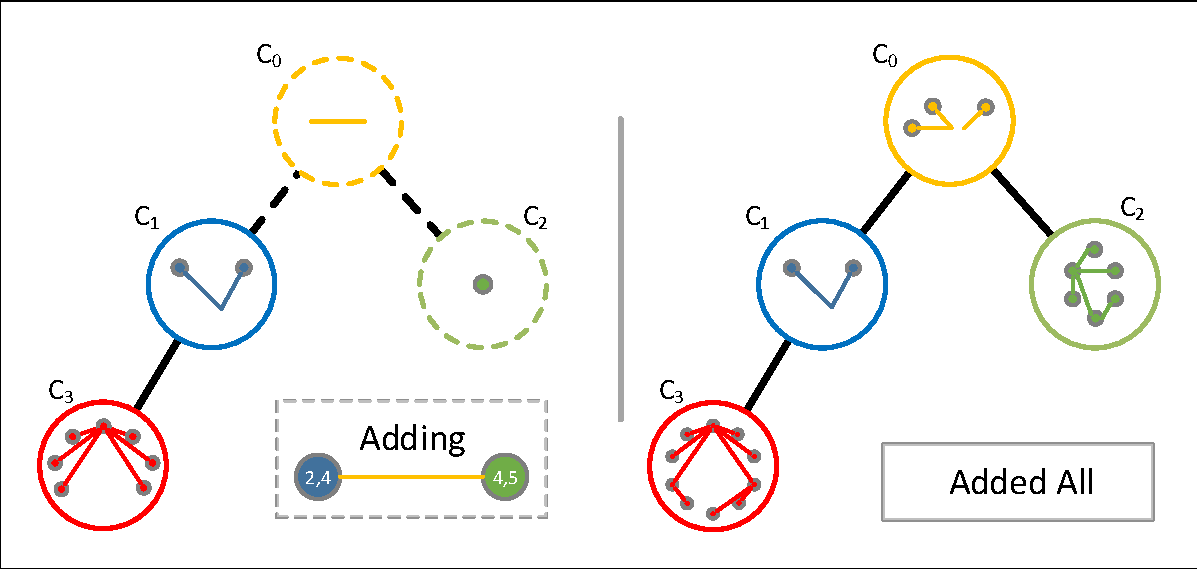
\includegraphics[width=\linewidth]{./figures/tree_index.pdf}
    \caption{An example \treeindex{} of the \inducedgraph{} in \autoref{fig:\inducedgraph{}}}
    \label{fig:\treeindex{}}
\end{figure}

\autoref{alg:\treeindex{}_construction} shows the procedure to build the \treeindex{} $G_t$. The algorithm uses BFS to traverse the \inducedgraph $G_m$. For each vertex $x$, if it does not have a parent vertex in the BFS traversal, then the algorithm uses it as a seed vertex to create a new index tree. Otherwise it is combined to the same index tree $T \in G_t$ as its parent vertex $y$. According to \autoref{thm:\inducedgraph{}_vertex_trussness}, we have the following equation.

\begin{equation}
w_{x} \ge w_{(x,y)}, w_{y} \ge w_{(x,y)}
\label{equ:lowest_edge_weight}
\end{equation}

An example is shown in \autoref{fig:\treeindex{}}

\begin{Thm}
For a vertex $x$ and its neighbor vertex $y$ in \inducedgraph{} $G_m$, if their representing edges in $G_o$ are contained in the same k-truss community with trussness of $k$, then $k \le w_{(x,y)}$. 
\label{thm:k_le_edge_weight}
\end{Thm}

\begin{proof}
Since $G_m$ is the maximum spanning forest, it has the cycle property, \ie for any cycle in $G_{m}^{\prime}$, if the weight of an edge in the cycle is smaller than the individual weights of all the other edges in the cycle, then this edge cannot belong to a maximum spanning forest. So there is no path in $G_{m}^{\prime}$ between $x$ and $y$ that has all edges with weight $> w_{(x,y)}$. Suppose $x$ and $y$ representing $e_x$ and $e_y$ in $G_o$, this means that $e_x$ is not triangle connected to $e_y$ through edges in $G_o$ with trussness $> w_{(x,y)}$. Therefore, it is not possible for $e_x$ and $e_y$ to exist in the same k-truss community with $k > w_{(x,y)}$.
\end{proof}
 
Having a parent $y$ in the BFS search only means that the vertex $x$ can be combined to the current index tree $T$. We still have a problem to solve: On which part of $T$ should the algorithm add the vertex $x$? According to \autoref{thm:k_le_edge_weight} and \autoref{equ:lowest_edge_weight}, the algorithm needs to backtrack $T$ from $C_{y}^{max}$ to find an ancestor vertex $C_a$ that meets $\tau_{C_a} \le w_{(x,y)}$ and use it as the merge point of $x$. We refer to the index vertices $C_{y}^{max},...,C_{i},...,C_{a}$ as the backtrack branch for vertex $x$ in $T$ and denote it as $B$. % If no such an index vertex $C_a$ can be found, \ie the algorithm reaches the root of $T$ and has not found a qualified ancestor vertex, it creates a new index vertex $C_{x}^{max}$ with trussness $\tau_{C_{x}^{max}} = w_{x}$ and uses it as the new root of $T$, \ie the algorithm attaches the old root of $T$ as a child vertex to $C_{x}^{max}$. \note{this part need to modify}

Once the algorithm has found $C_a$, it needs to check the relations of $\tau_{C_a}$, $w_{(x,y)}$ and $w_{x}$ to decide how to merge vertex $x$ to $T$. Note that they follow $\tau_{C_a} \le w_{(x,y)} \le w_{x}$, so we have 4 cases shown in \autoref{alg:\treeindex{}_construction}. As long as $\tau_{C_a} \neq w_{x}$, we create a new index vertex $C_{x}^{max}$ with trussness $\tau_{C_{x}^{max}} = w_{x}$. If $\tau_{C_a} < w_{(x,y)} < w_{x}$, we also create a new index vertex $C_{(x,y)}$ with trussness $\tau_{C_{(x,y)}} = w_{(x,y)}$. Then we adjust the tree structure of $T$ with new index vertices. Finally, we update the hash table to record in which index vertex $x$ is.
% If there is a child index vertex of $C_a$ on backtrack branch $B$, we denote it as $C_c$, and we have $\tau_{C_c} > w_{(x,y)}$. We have the following 4 cases:

%\begin{itemize}
	%\item $\tau_{C_a} < w_{(x,y)}$
	%\begin{itemize}
		%\item $w_{(x,y)} = w_{x}$: \\
		%Create a new index vertex $C_{x}^{max}$ with trussness $\tau_{C_{x}^{max}} = w_{x}$, and attach it to $T$ as a child vertex of $C_a$. Attach $C_c$ to $C_{x}^{max}$ as a child vertex since $\tau_{C_{x}^{max}} = w_{x} = w_{(x,y)} < \tau_{C_c}$. Update the hash table $h[x] = C_{x}^{max}$.
		%\item $w_{(x,y)} < w_{x}$: \\
		%Create a new index vertex $C_{x}^{max}$ with trussness $\tau_{C_{x}^{max}} = w_{x}$. Create another index vertex $C_{(x,y)}$ with trussness $\tau_{C_{(x,y)}} = w_{(x,y)}$. Attach the index vertex $C_{(x,y)}$ to $C_a$ as a child and attach both $C_{x}^{max}$ and $C_c$ as two separate children to the index vertex $C_{(x,y)}$. Update the hash table $h[x] = C_{x}^{max}$.
	%\end{itemize}
	%\item $\tau_{C_a} = w_{(x,y)}$
	%\begin{itemize}
		%\item $w_{(x,y)} = w_{x}$: \\
		%Update the hash table $h[x] = C_{a}$.
		%\item $w_{(x,y)} < w_{x}$: \\
		%Create a new index vertex $C_{x}^{max}$ with trussness $\tau_{C_{x}^{max}} = w_{x}$. Attach it to $T$ as a separate child to $C_a$ along side with $C_c$. Update the hash table $h[x] = C_{x}^{max}$.
	%\end{itemize}
%\end{itemize}

For each vertex of $G_m$, the backtrack procedure takes $O(k_{max})$ time, where $k_{max}$ is the highest trussness of any k-truss community in $G_o$. Since the index construction process is a BFS on a maximum spanning tree, the \treeindex{} construction algorithm takes $O(k_{max}m)$ time. As each vertex in $G_t$ represents a k-truss community in $G_o$, and $G_t$ is a forest. The algorithm takes $O(m)$ space and the index size is also $O(m)$ space. Although in practice, the size of $G_t$ is much smaller than $O(m)$.

%\begin{Thm}
%When $\tau{A} < \tau{e}$, the vertex $u$ only connects to this branch of index vertex $A$ with currently discovered edges, not other branches.
%\end{Thm}
%
%\begin{proof}
%If it want connect to other branches, it need to connect through ancestors. But $A$ has a lower trussness that can not connect higher k truss communities.
%\end{proof}

\vskip 0.1in \noindent \textbf{Query on \TreeIndex{}.}
\Treeindex{} supports three basic types of k-truss community queries of a single query vertex $q$ as listed below.

\begin{itemize}
	\item{K-truss query:} Given a vertex $q$ and an integer $k$, find the k-truss community that contains $q$.
	\item{Max-k-truss query:} Given a vertex $q$, find the k-truss community with highest possible trussness that contains $q$.
	\item{Any-k-truss query:} Given a vertex $q$, find all the k-truss communities that contains $q$.
\end{itemize}

Max-k-truss query is naturally supported by simply looking up the hash table $h$ and comparing trussness of $h[x_e]$ for each neighbor edge. We show the queries process algorithms for k-truss query and any-k-truss query in \autoref{alg:\treeindex{}_query}. A common operation used in both query algorithms is what we called backtrack branch search, which is defined in \autoref{def:backtrack_branch_search} below. We can see that if a specific $k$ is provided, the backtrack branch search will stop once the trussness falls below $k$. On the other hand, if no $k$ is provided, a value of $0$ is used and the search will reach the root of the tree.

\begin{Def}[Backtrack branch search]
Given a vertex $C_{0} \in G_t$ and an integer $k$, the backtrack branch search returns a list of vertices $C_{0},...,C_{i},...$ that $C_{i+1}$ is the parent vertex of $C_{i}$ in $G_t$ and any vertex $C_{i}$ meets $\tau_{C_{i}} \ge k$. We refer to the searching results $C_{0},...,C_{i},...$ as backtrack branch and denote it as $B$.
\label{def:backtrack_branch_search}
\end{Def}

\Treeindex{} also supports all three types of queries when the input is a set of query vertices $Q$. The query process algorithms simply takes intersections of the query results of each individual query vertex for k-truss queries and any-k-truss queries. For max-k-truss queries, the query process algorithm needs to calculate the least common ancestors in $G_t$ of the results of each individual query vertex.

\begin{algorithm}
	\KwData{$G_{o}(V_{o},E_{o})$, $G_{t}(V_{t},E_{t})$, the hash table $h$, a query vertex $q$ or a set of query vertices $Q$, [an integer k]}
	\KwResult{a set of k-truss community IDs $R$}
	\SetKwProg{Fn}{function}{}{end}
	\BlankLine
	\Fn{branch\_search ($C \in G_t$, $G_t$, [$k$ = 0])}{
		$B \gets \emptyset$\;
		\While{$C \neq \emptyset$ \textbf{and} $\tau_{C} \ge k$}{
			$B \gets B \bigcup {C}$\;
			$C \gets C.parent$\;
		}
		\Return{$B$}
	}
	\BlankLine
	\Fn{query\_k ($q$, $G_o$, $G_t$, $k$)}{
		$R \gets \emptyset$\;
		\For{$e \in N_q$}{
			$B \gets$ branch\_search ($h[x_e]$, $G_t$, $k$)\;
			\If{$\tau_{B[-1]} = k$}{
				$R \gets R \bigcup B[-1]$; \Comment{$B[-1]$ is the last element in $B$}
			}
		}
		\Return{$R$}
	}
	\BlankLine
	\Fn{query\_anyk ($q$, $G_o$, $G_t$)}{
		$R \gets \emptyset$\;
		\For{$e \in N_q$}{
			$B \gets$ branch\_search ($h[x_e]$, $G_t$)\;
			$R \gets R \bigcup B$\;
		}
		\Return{$R$}
	}
	\caption{Query on \Treeindex{}}\label{alg:\treeindex{}_query}
\end{algorithm}

For single vertex queries, the time complexity is $O(d_q)$ for max-k-truss queries and $O(\sum_{e \in N_q}\tau_{h[x_e]})$ for k-truss and any-k-truss queries. The space complexity is $O(1)$ for max-k-truss queries, $O(d_q)$ for k-truss queries and $\sum_{e \in N_q}\tau_{h[x_e]}$ for any-k-truss queries. For multiple vertices max-k-ktruss queries, since the least common ancestor computation takes $O(H)$\footnote{$O(H)$ is for simple online algorithm, off-line algorithms can achieve time complexity of $O(1)$~\cite{bender2000lca}.} time, where $H$ is the height of the tree. The query time is $O(\sum_{q \in Q}(\max_{e \in N_q}\tau_{h[x_e]} + d_q))$ and the space is $O(\max_{q \in Q}\max_{e \in N_q}\tau_{h[x_e]})$. Multiple vertices k-truss queries take $O(\sum_{q \in Q}\sum_{e \in N_q}\tau_{h[x_e]})$ time and $O(\max_{q \in Q}d_q)$ space. For multiple vertices any-k-truss queries, the time and space complexity is $O(\sum_{q \in Q}\sum_{e \in N_q}\tau_{h[x_e]})$ and $O(\max_{q \in Q}\sum_{e \in N_q}\tau_{h[x_e]})$ respectively.

%\Treeindex{} supports multiple types of k-truss community queries. We start by defining backtrack branch search and least common ancestor. Then we introduce four most common types of queries supported by \treeindex{}.
%
%\begin{Def}[Backtrack branch search]
%Given a vertex $C_{0} \in G_t$ and an integer $k$, the backtrack branch search returns a list of vertices $C_{0},...,C_{i},...$ that $C_{i+1}$ is the parent vertex of $C_{i}$ in $G_t$ and any vertex $C_{i}$ meets $\tau_{C_{i}} \ge k$. We refer to the searching results $C_{0},...,C_{i},...$ as backtrack branch and denote it as $B$.
%\label{def:backtrack_branch_search}
%\end{Def}
%
%\begin{Def}[Least common ancestor]
%Given a set of vertices $C_{0},...,C_{s}$ in $G_t$, if $C_{0},...,C_{s}$ belong to the same tree $T$, the least common ancestor of $C_{0},...,C_{s}$ is the vertex furthest from the root of $T$ that is an ancestor of all vertices in $C_{0},...,C_{s}$. We denote the least common ancestor as the $LCA$.
%\label{def:lca_search}
%\end{Def}
%
%\Treeindex{} supports both single vertex query and multiple vertices query. It also support query for k-truss communities of a specific $k$ or any possible $k$. Here we list four most common types of queries supported by \treeindex{}.
%
%\begin{itemize}
	%\item \textbf{Single vertex and a specified $k$.} \\
	%Given a query vertex $q$ and an integer $k$, find the k-truss community that contains $q$ with trussness $k$. The query algorithm iterates neighbor edges of $q$. For each edge $e$, let $x_e$ be the representing vertex in $G_m$. The algorithm performs a backtrack branch search with $h[x_e]$ and $k$ in $G_t$ and get the backtrack branch $B_e$. Let $C_e$ contain the last vertex in $B_e$ if it has trussness equals $k$ or be $\emptyset$ otherwise. The union of results of all neighbor edges $\bigcup_{e} C_e$ is all the k-truss communities that contains $q$ with trussness of $k$. 
	%\item \textbf{Single vertex with any possible $k$.} \\
	%Given a query vertex $q$, find all the k-truss communities that contains $q$. Similar to last one, the query algorithm also performs a backtrack branch search on each neighbor edge of $q$. The union of results of all neighbor edges $\bigcup_{e} B_e$ are all the k-truss communities that contains $q$. 
	%\item \textbf{Multiple vertex with a specified $k$.} \\
	%Given a set of query vertices $Q$, find the k-truss community that contains all vertices in $Q$ with trussness $k$. For each $q \in Q$, find $R_q = \bigcup_{e} C_e$ using the single vertex query algorithm. The intersection of results of all query vertices $\bigcap_{q} R_q$ is all the k-truss communities that contains all vertices in $Q$ with trussness of $k$.
	%\item \textbf{Multiple vertex with any possible $k$.} \\
	%Given a set of query vertices $Q$, find all k-truss communities that contains all vertices in $Q$. For each $q \in Q$, let $e_q$ be neighbor edges of $q$ and $x_{e_q}$ be the representing vertex in $G_m$. We denote $\bigcup_{e_q} h[x_{e_q}]$ as $H_q$. For two vertices $p,q \in Q$, the query algorithm combines $H_p$ and $H_q$ in the following way. For each pair of vertices $h[x_{e_p}] \in H_p$ and $h[x_{e_q}] \in H_q$, the algorithm finds the least common ancestor of $h[x_{e_p}]$ and $h[x_{e_q}]$ in $G_t$, if there is any. We denote it as $LCA_{\{e_{p},e_{q}\}}$. The union of least common ancestor of each pair of vertices $H_{\{p,q\}} = \bigcup_{\{e_{p},e_{q}\}} LCA_{\{e_{p},e_{q}\}}$ is the combining result of $H_p$ and $H_q$. The algorithm iteratively combines all query vertices in this way and gets $H_Q$. Then for each index vertex in $H_Q$, the algorithm performs a backtrack branch search to and return the union of the results $R_Q$ which is all the k-truss communities that contains all vertices in $Q$. 
%\end{itemize}

%\begin{algorithm}
	%\KwData{$G_{o}(V_{o},E_{o})$, $G_{t}(V_{t},E_{t})$, the hash table $h$, a query vertex $q$ or a set of query vertices $Q$, [an integer k]}
	%\KwResult{a set of k-truss community IDs $R$}
	%\SetKwProg{Fn}{function}{}{end}
	%\BlankLine
	%\Fn{branch\_search ($C \in G_t$, $G_t$, [$k$ = 0])}{
		%$B \gets \emptyset$\;
		%\While{$C \neq \emptyset$ \textbf{and} $\tau_{C} \ge k$}{
			%$B \gets B \bigcup {C}$\;
			%$C \gets$ parent of $C$ in $G_t$\;
		%}
		%\Return{$B$}
	%}
	%\BlankLine
	%\Fn{query\_singleq ($q$, $G_o$, $G_t$, $k$)}{
		%$R \gets \emptyset$\;
		%\For{$e \in N_q$}{
			%$B$ = branch\_search ($h[x_e]$, $G_t$, $k$)\;
			%\If{$\tau_{B[-1]} = k$}{
				%$R \gets R \bigcup B[-1]$; \Comment{$B[-1]$ is the last element in $B$}
			%}
		%}
		%\Return{$R$}
	%}
	%\BlankLine
	%\Fn{query\_singleq\_anyk ($q$, $G_o$, $G_t$)}{
		%$R \gets \emptyset$\;
		%\For{$e \in N_q$}{
			%$B$ = branch\_search ($h[x_e]$, $G_t$)\;
			%$R \gets R \bigcup B$\;
		%}
		%\Return{$R$}
	%}
	%\BlankLine
	%\Fn{query\_multiq ($Q$, $G_o$, $G_t$, $k$)}{
		%$R \gets \emptyset$, $initialized \gets False$\;
		%\For{$q \in Q$}{
			%\eIf{$initialized = False$}{
				%$R \gets$ query\_singleq ($q$, $G_o$, $G_t$, $k$)\;
				%$initialized \gets True$\;
			%}{
				%$R \gets R \bigcap$ query\_singleq ($q$, $G_o$, $G_t$, $k$)\;
			%}
		%}
		%\Return{$R$}
	%}
	%\BlankLine
	%\Fn{query\_multiq\_anyk ($Q$, $G_o$, $G_t$)}{
		%$R \gets \emptyset$, $initialized \gets False$\;
		%\For{$q \in Q$}{
			%\eIf{$initialized = False$}{
				%$R \gets$ query\_singleq\_anyk ($q$, $G_o$, $G_t$)\;
				%$initialized \gets True$\;
			%}{
				%$R^{\prime} \gets$ query\_singleq\_anyk ($q$, $G_o$, $G_t$)\;
			%}
		%}
		%\Return{$R$}
	%}
	%\caption{Query on \inducedgraph{}}\label{alg:\inducedgraph{}_query}
%\end{algorithm}
%
%For single vertex queries, the time complexity is $O(\sum_{e \in N_q}\tau_{h[x_e]})$, the space complexity is $O(d_q)$ if $k$ is specified or $\sum_{e \in N_q}\tau_{h[x_e]}$ otherwise. For multiple vertices queries, when $k$ is specified, the time complexity is $O(\sum_{q \in Q}\sum_{e \in N_q}\tau_{h[x_e]})$ and the space complexity is $O(\sum_{q \in Q}d_q)$. Since the least common ancestor computation takes $O(h)$\footnote{$O(h)$ is for simple online algorithm, off-line algorithms can achieve time complexity of $O(1)$~\cite{bender2000lca}.} time, where $h$ is the height of the tree. If $k$ is not specified, the time complexity is $O(\sum_{q \in Q}\sum_{e \in N_q}\tau_{h[x_e]})$ and the space complexity is $O(\sum_{q \in Q}\sum_{e \in N_q}\tau_{h[x_e]})$.
